\documentclass{article}

\usepackage{ctex}
\usepackage{graphicx}
\usepackage{float}
\usepackage{datetime}
\usepackage{amssymb}
\usepackage{setspace}
\usepackage{amsmath}
\usepackage{geometry}
\usepackage{tikz}
\usetikzlibrary{positioning} %为了实现相对位置的设定
\usepackage{xcolor} %为了实现不同的颜色
\usepackage{listings}
\usepackage{qtree}% 绘制语法分析树
\usepackage{forest}% 绘制语法分析树
\lstset{
    numbers=left, 
    numberstyle= \tiny, 
    keywordstyle= \color{ blue!70},
    commentstyle= \color{red!50!green!50!blue!50}, 
    frame=shadowbox, % 阴影效果
    rulesepcolor= \color{ red!20!green!20!blue!20} ,
    escapeinside=``, % 英文分号中可写入中文
    xleftmargin=2em,xrightmargin=2em, aboveskip=1em,
    framexleftmargin=2em
} 

\geometry{left=3.0cm,right=2.0cm,top=2.5cm,bottom=2.5cm}
\title{离散数学 Problem Set 11}
\renewcommand{\baselinestretch}{1.5} %调整行间距
\tikzstyle{startstop} = [rectangle, rounded corners, minimum width=3cm, minimum height=1cm,text centered, draw=black]
\tikzstyle{decision} = [diamond, draw, text width=5.5em, text badly centered, inner sep=0pt]
\tikzstyle{process} = [rectangle, minimum width=3cm, minimum height=1cm, text centered, draw=black]
\tikzstyle{arrow} = [thick,->,>=stealth]
\tikzset{
    bnode/.style ={
    circle, %矩形节点
    minimum width =20pt, %最小宽度
    minimum height =20pt, %最小高度
    inner sep=5pt, %文字和边框的距离
    draw=blue, %边框颜色}
    fill=black,
    text=white
    }
}
\tikzset{
    rnode/.style ={
    circle, %矩形节点
    minimum size =20pt, %最小宽度
    % max size = 25pt,
    inner sep=5pt, %文字和边框的距离
    draw=blue, %边框颜色}
    fill=red,
    text=white
    }
}
\tikzset{
    leaf/.style={
    rectangle,
    minimum size =20pt, %最小宽度
    inner sep=5pt, %文字和边框的距离
    draw=blue, %边框颜色}
    fill=white,
    text=black
    }
}
\tikzset{
    fa/.style={
    circle,
    minimum size =20pt, %最小宽度
    inner sep=5pt, %文字和边框的距离
    draw=blue, %边框颜色}
    fill=white,
    text=black
    }
}
\tikzset{
    enode/.style ={
    circle, %矩形节点
    minimum size =5pt, %最小宽度
    inner sep=5pt, %文字和边框的距离
    draw=blue, %边框颜色}
    fill=black,
    text=white
    }

    
}
\geometry{left=3.0cm,right=2.0cm,top=2.5cm,bottom=2.5cm}
\title{离散数学作业 Problem Set 10}
\renewcommand{\baselinestretch}{1.5} %调整行间距

\author{201830099 周义植}
\date{\today}

\begin{document}
\maketitle
\section*{Problem 1}
证明:

无回路的简单连通图即为树。对每个叶子节点,其父节点一定只有其一个子节点为叶子节点(否则无法形成完美匹配)。匹配所有叶子节点和其父节点,
又会得到若干不连通的树。如此反复进行,每次匹配的方法都唯一(叶子节点一定只能和父节点匹配),直到所有的点都被匹配或有的点无法匹配。
该方案唯一,所以无回路的简单连通图最多存在一种完美匹配的方式。


\section*{Problem 2}
证明:

将图染成黑白两色,相邻块的颜色不同。如此每个小矩形一定占据一个黑块和一个白块。但是按该方法染下的黑白两色不一样多,因此无法用小矩形盖住。

\section*{Problem 3}

证明:

设二部图的两个点集大小为x,n-x.完全二部图的情况下边数最多,所以

\begin{equation}
    \nonumber
    m \leq x(n-x) \leq \frac{(x+n-x)^2}{4} = \frac{n^2}{4}
\end{equation}

\section*{Problem 4}
证明:

构造二部图$G = (V_1,V_2,E)$,$V_1$中的每个顶点表示一种k划分的每个子集,$V_2$中的每个顶点表示另一种划分的每个子集,若两个子集有公共元素,则两点相邻。
易知$\forall A\subseteq  V_1,|N(A)|\geq |A|$,因为A包含的元素所有共同元素的集合一定大于A本身。由Hall定理存在饱和匹配,而两个点集大小相同,因此有完全匹配。
将完全匹配中每条边的两个顶点取一个公共元素,则构成一个共同的代表集。
\section*{Problem 5}
证明:

取任意一个点为起点,除去该点后将图按problem 2的方式染色,分为二部图$(V_1,V_2,E)$,因为N,M均为奇数,$|V_1|=|V_2|+1$(被取掉的点在$V_1$)。除去起点取该图的最大匹配,则存在哈密顿回路等价于存在该匹配的增广路径(从该未饱和点开始再由该未饱和点结束)。而由Berge定理,矛盾。因此该图不存在哈密顿回路。

\section*{Problem 6}
\subsection*{1}
上界:$4(m-1)+1 = 81,m=21$

下界:$m^4=81,m=3$

\subsection*{2}
由$\lceil log_ml\rceil = h,m=3$

\section*{Prolem 7}
三个顶点:3种。三个顶点的树只有$P_3$一种结构,两个树不同构当且仅当中间的点标记不同,共三种。

四个顶点:有$P_4,K_{1,3}$两种结构,前者有$4!/2=12$种,后者有4种,共16种。

\section*{Problem 8}
设其由x个度数为1的顶点,则$\Sigma deg(v) = x+\Sigma i*(n_i)$又有该图的边数$m = x+\Sigma (n_i)-1$

又有$2m = \Sigma deg(v),$因此$x = \Sigma(i-2)*n_i+2$
\section*{Problem 9}
证明:

边数$m=n-1=2n_2+n_1,$因此$n_0=n_2+1$

当只有度数为0或1的点时,$n=n_0+n_2=2*n_2+1,$一定是奇数;

$t=n_0=\frac{n+1}{2}$


\section*{Problem 10}

\begin{figure}[H]
    \centering
    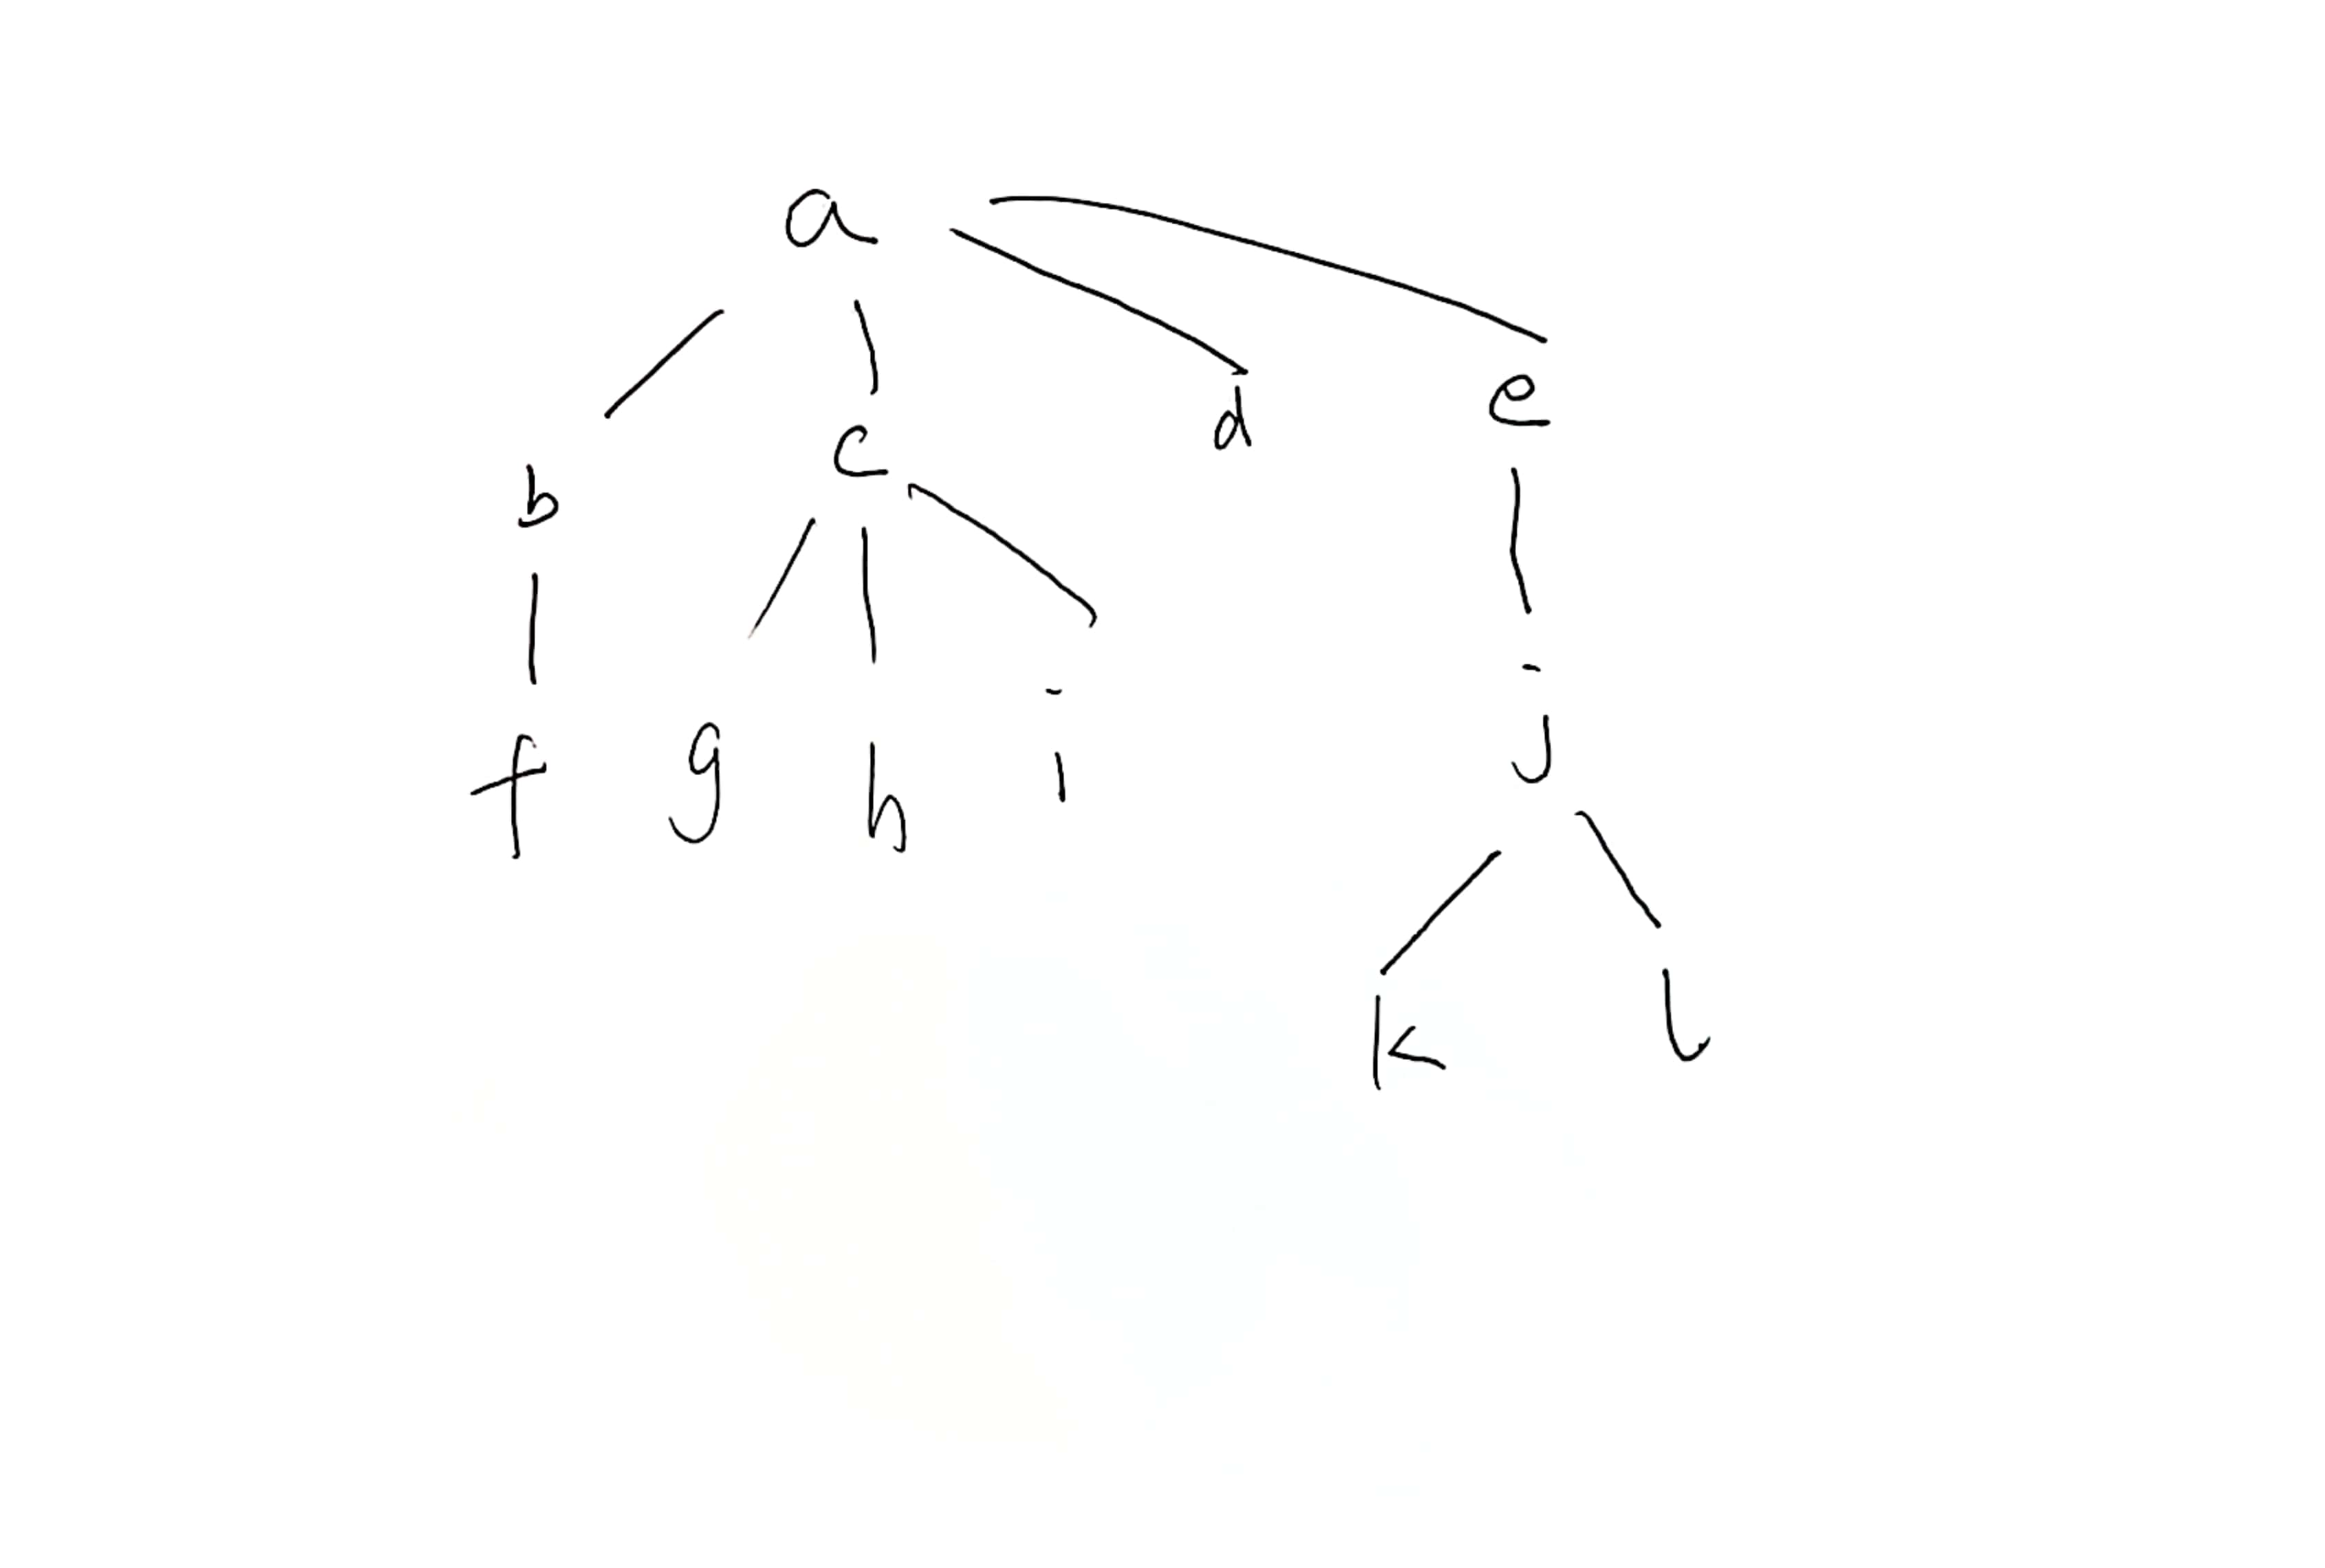
\includegraphics[scale=0.2]{p2.jpg}
\end{figure}

\end{document}